\documentclass[12pt,a4paper,openright,twoside]{book}
\usepackage[utf8]{inputenc}
\usepackage{disi-thesis}
\usepackage{code-lstlistings}
\usepackage{notes}
\usepackage{shortcuts}
\usepackage{acronym}
\usepackage[acronym]{glossaries}

\school{\unibo}
\programme{Corso di Laurea Triennale in Ingegneria e Scienze Informatiche}
\title{Uso del Machine Learning per bloccare siti DGA}
\author{Simone Collorà}
\date{\today}
\subject{Programmazione a Oggetti}
\supervisor{Prof. Mirko Viroli}
\cosupervisor{Dott. CoSupervisor 1}
\morecosupervisor{Dott. CoSupervisor 2}
\session{I}
\academicyear{2024-2025}

% Definition of acronyms
\acrodef{IoT}{Internet of Thing}
\acrodef{vm}[VM]{Virtual Machine}
\newacronym{DGA}{DGA}{Domain Generation Algorithm}
\newacronym{C&C}{C\&C}{Command and Control}
\newacronym{P2P}{P2P}{Peer to Peer}
\newacronym{IRC}{IRC}{Internet Relay Chat}


\mainlinespacing{1.241} % line spacing in mainmatter, comment to default (1)

\begin{document}
\frontmatter\frontispiece
\nocite{*}

\begin{abstract}	
Max 2000 characters, strict.
\end{abstract}

\begin{dedication} % this is optional
Optional. Max a few lines.
\end{dedication}

%----------------------------------------------------------------------------------------
\tableofcontents   
\listoffigures     % (optional) comment if empty
\lstlistoflistings % (optional) comment if empty
%----------------------------------------------------------------------------------------

\mainmatter

%----------------------------------------------------------------------------------------
\chapter{Introduzione}
\label{chap:introduction}
%----------------------------------------------------------------------------------------

La sicurezza informatica è un argomento di crescente importanza
nel mondo moderno. Con il passare del tempo,
i sistemi di protezione sono diventati sempre più sofisticati
e potenti ma, allo stesso tempo, anche gli hackers 
hanno sviluppato tecniche sempre più avanzate per eludere i sistemi di protezione.
Tra queste vi è sicuramente l'uso di Botnets
dei \acrfull{C&C} servers. I \acrshort{C&C} sono dei server che manipolano
i computer infetti da malwares, i Botnets, permettendo
all'attaccante di eseguire codice malevolo da remoto.
Il malware, però, deve conoscere un indirizzo IP o un dominio
per contattare il server. L'attaccante potrebbe
inserire in modo bruto l'indirizzo IP del server nel codice del malware,
ma questo metodo è facilmente rilevabile e bloccabile.
Gli hackers, quindi, preferiscono utilizzare dei domini
generati in modo pseudo casuale per nascondere i loro server chiamati
\acrfull{DGA} servers. Negli ultimi anni, sono stati sviluppati
vari metodi di Machine Learning per rilevare questi domini.



\paragraph{Struttura della tesi}
Il lavoro di tesi si dividerà in 4 capitoli. Nel primo
capitolo verrano descritti concetti di base riguardanti DNS, \acrshort{DGA} e Botnets,
e Machine Learning con una breve descrizione delle reti neurali e di alcuni
algoritmi usati. Nel secondo capitolo verrà descritto il progetto,
i suoi obiettivi e i risultati ottenuti. Nell'ultimo capitolo
verranno discusse le conclusioni e i possibili sviluppi futuri.

%\note{At the end, describe the structure of the paper}

\chapter{Uso del Machine Learning per rilevare i DGA}

\section{Botnets e DGA}
%I suggest referencing stuff as follows: \cref{fig:DGA example} or \Cref{fig:DGA example}

\subsection{Botnets}

I Botnets sono reti di computer infetti da malware, chiamati bot,
che possono essere controllati da un attaccante, il botmaster.
La vita di un botnet di solito sono questi:
\begin{enumerate}
    \item \textbf{Infezione e propagazione}: Questo è il primo
    passaggio. L'attaccante cerca di infettare un computer
    tramite vari metodi come email con link malevoli o \acrfull{P2P} sharing.
    Una volta infettato un dispositivo, il malware cerca di infettare
    altri dispositivi nella rete.

    \item \textbf{Rallying}: i bots cercano di contattare per la prima volta
    il server \acrshort{C&C} per far capire all'attaccante
    che l'attacco è andato a buon fine.

    \item \textbf{Commands and Reports}: il malware esegue le istruzioni
    ricevute dal server \acrshort{C&C} e invia i risultati al botmaster.
    I bots ascoltano i comandi dal server \acrshort{C&C} 
    o si connettono ad esso periodicamente. Appena ricevono
    un comando lo eseguono, inviano i risultati al botmaster
    e aspettano un nuovo comando.

    \item \textbf{Abbandono}: Quando un bot non è più utile o utilizzabile,
    il botmaster può decidere di abbandonarlo. Il botnet, invece,
    sarà completamente distrutto quando tutti i bot saranno
    abbandonati o bloccati dalla vittima o quando il \acrshort{C&C} server
    verrà bloccato


\end{enumerate}

\begin{figure}
    \centering
    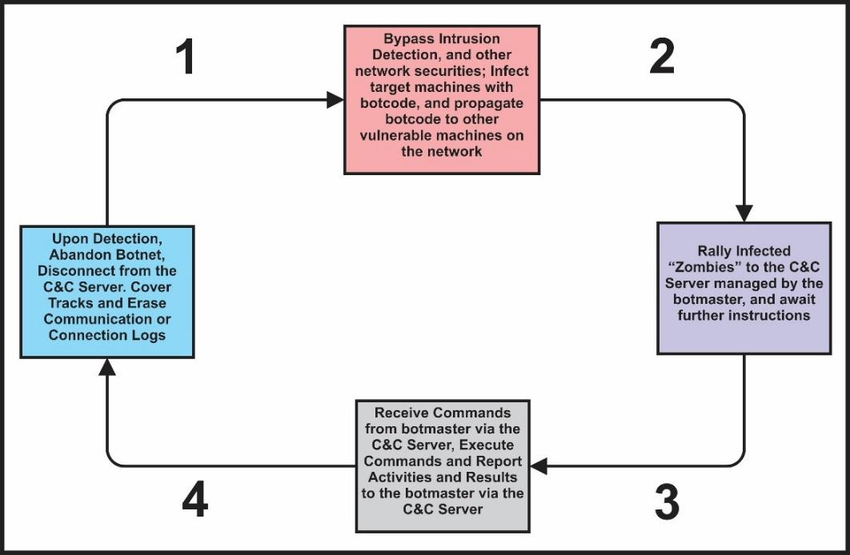
\includegraphics[width=.8\linewidth]{figures/The-Lifecycle-Schema-of-a-typical-Botnet.png}
    \caption{Ciclo di vita di un botnet \cite{Ogu2016}}
    \label{fig:botnet}
\end{figure}

\subsection{Command and Control} 

Il meccanismo del \acrshort{C&C} crea un canale di comunicazione
tra il botmaster e i bot. Questo è essenziale per il funzionamento
del botnet. Ci sono tre tipi di server \acrshort{C&C}:

\begin{itemize}
    \item \textbf{Centralizzati}: In questo tipo di server, il botmaster
    controlla tutti i bot tramite un server centrale. Questo è il metodo
    più semplice e veloce per controllare i bot ma è anche il più vulnerabile.
    Se il server centrale viene bloccato, tutti i bot non possono più
    ricevere comandi. Questo a sua volta è diviso in due categorie:
    \begin{itemize}
        \item \textbf{IRC} : \acrfull{IRC} è un sistema di chat
        usato per comunicare tra i bot e il botmaster in tempo reale.
        Questo era più usato nella prima generazione di botnet. 
        I bot si connettono al server \acrshort{IRC} e aspettano
        i comandi dal botmaster. I bot seguono un approccio PUSH ovvero
        quando un bot si connette ad un determinato canale, esso rimane connesso.
        \item \textbf{HTTP}: Il più usato. Con questa tecnica, i bot usano un URL o IP
        per contatattare il server \acrshort{C&C}. Qua invece i bot seguono
        un approccio PULL. I bot si connettono al server \acrshort{C&C}
        periodicamente e controllano se ci sono nuovi comandi. Questo processo
        va ad intervalli regolari definiti dal botmaster.
    \end{itemize}

    \item \textbf{Decentralizzati}: Questo tipo di \acrshort{C&C}
    è basato su un sistema \acrshort{P2P} senza un server centrale. In questo modo,
    computer infetti fanno sia da bot che da server \acrshort{C&C}.
    Questo metodo è più difficile da rilevare ma anche
    più complesso da implementare \cite{4804459}.

\end{itemize}

\begin{figure}
    \centering
    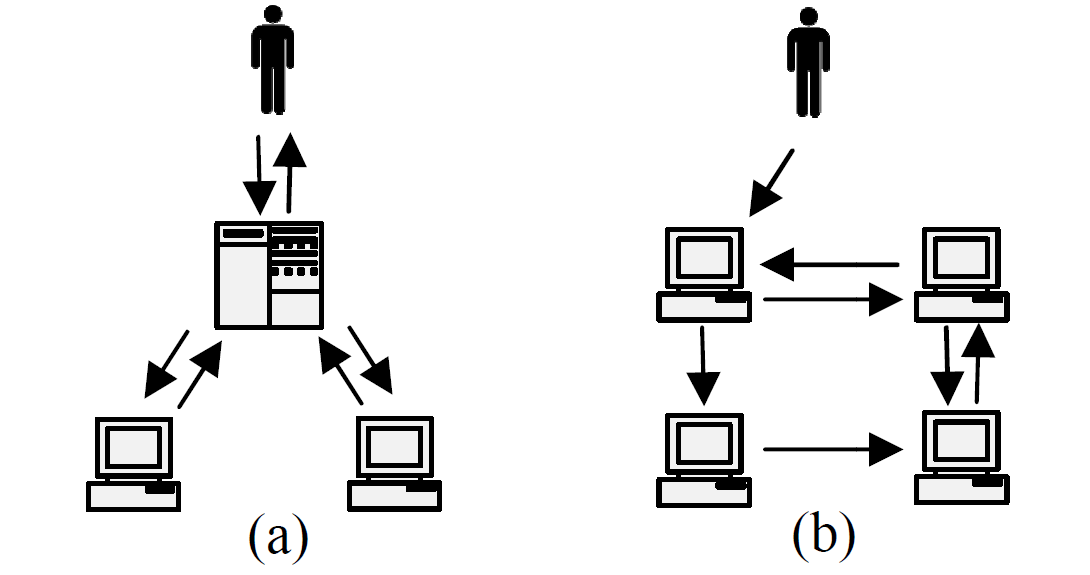
\includegraphics[width=.8\linewidth]{figures/Types-of-CC.png}
    \caption{Esempio di server \acrshort{C&C}. (a) centralizzato, (b) decentralizzato \cite{6487169}}
    \label{fig:command and control}
\end{figure}

\subsection{Domain Generation Algorithm}


I \acrshort{DGA} sono algoritmi che generano migliaia di domini in modo pseudo casuale.
Prima viene scelto un seed, di solito la data odierna
o anche le previsioni meteo \cite{8621875} e, tramite
un algoritmo di hashing, vengono generati i domini.
Questi domini vengono poi utilizzati per contattare i server \acrshort{C&C}.
Non tutti i domini generati però sono registrati.
Il computer infetto, tramite i DNS locali, cercherà di tradurre
un dominio in un indirizzo IP.
Se non riesce a contattarlo con un determinato dominio,
proverà con il successivo finché non troverà
un dominio valido che permetterà al malware di comunicare con
il server \acrshort{C&C} \cite{8489147}.
In questo modo, diventa più difficile per i sistemi di protezione
rilevare e bloccare i loro attacchi.
Si potrebbe pensare di bloccare direttamente i domini tramite
una blacklist ma questo metodo
risulta inefficace poiché vengono generati migliaia di domini
continuamente. Si pensi che Conficker C, un famoso malware
che utilizza \acrshort{DGA}, è in grado di generare
fino a 50.000 domini pseudo casuali al giorno \cite{978131}.

Un altro modo per contrastare ciò
potrebbe essere quello di fare reverse engineering
del \acrshort{DGA} per capire quale seed viene utilizzato per generare i domini.
Questo però risulta lento e dispendioso e possibilmente inefficace \cite{8887881}.

\begin{figure}
    \centering
    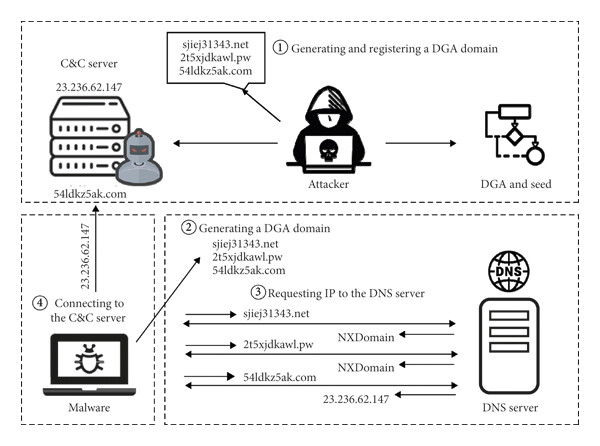
\includegraphics[width=.8\linewidth]{figures/DGA example.jpg}
    \caption{esempio del funzionamento di un \acrshort{DGA}}
    \label{fig:DGA example}
\end{figure}

Per contrastare i \acrshort{DGA}, sono stati sviluppati
vari metodi di Machine Learning in grado di rilevare i domini generati.
Questi metodi hanno due lati poisitivi:
\begin{itemize}
    \item Non richiedono un lungo processo di reverse engineering.
    \item Essendo l'AI una blackbox, è molto difficile
    per gli hackers eseguire un reverse engineering del modello.
\end{itemize}

\section{Machine Learning}
Il Machine Learning è una branca dell'informatica che punta
a far ragionare le macchine come gli esseri umani, ovvero
a svolgere compiti autonomamente senza essere programmati
esplicitamente e migliorando le loro prestazioni con l'esperienza
e i dati.
Abbiamo vari tipi di Machine Learning:
\begin{itemize}
    \item \textbf{Supervised Learning}: È la tecnica più comune
    per allenare le reti neurali \cite{ayodele2010types}. In questo tipo di apprendimento,
    il modello viene addestrato su un dataset etichettato. Un esempio
    di uso di questo tipo di apprendimento è la classificazione
    di immagini.
    \item \textbf{Unsupervised Learning}: In questo tipo di apprendimento,
    il modello, deve scoprire dei pattern o delle relazioni
    senza avere nessuna etichetta. Il modello deve trovare
    degli oggetti che condividono delle caratteristiche simili, chiamati
    cluster
    \item \textbf{Reinforcement Learning}: In questo tipo di apprendimento,
    ogni azione ha un effetto nell'ambiente che può essere positivo
    o negativo.
\end{itemize}




\subsection{Reti Neurali}

Una \textbf{Rete Neurale} o in inglese \textbf{Artificial Neural Network} (ANN) è il nome
di una branca dell'intelligenza artificiale che mira a simulare il
funzionamento del cervello umano \cite{zou2009overview}.
Il cervello umano è composto da miliardi di neuroni
che comunicano tra di loro tramite sinapsi.
Con le reti neurali artificiali, il funzionamento
è analogo. A livello matematico, un neurone artificiale è composto principalmente
da tre componenti:
\begin{itemize}
    \item \textbf{Pesi}: I pesi(weight in inglese) sono valori numerici che
    aiutano ogni nodo della rete neurale a determinare
    l'importanza di un input. Usando i pesi, il neurone
    può decidere se un input è importante o meno.
    \item \textbf{Funzione di attivazione}: la funzione di attivazione del neurone è la funzione
    che in input prende la sommatoria dei dati pesati con i pesi descritti in
    precedenza e produce un output che verrà poi inviato ad altri neuroni come
    input. Alcune delle funzioni di attivazione più comuni sono la funzione
    sigmoide e la funzione ReLU.
\end{itemize}

\begin{figure}
    \centering
    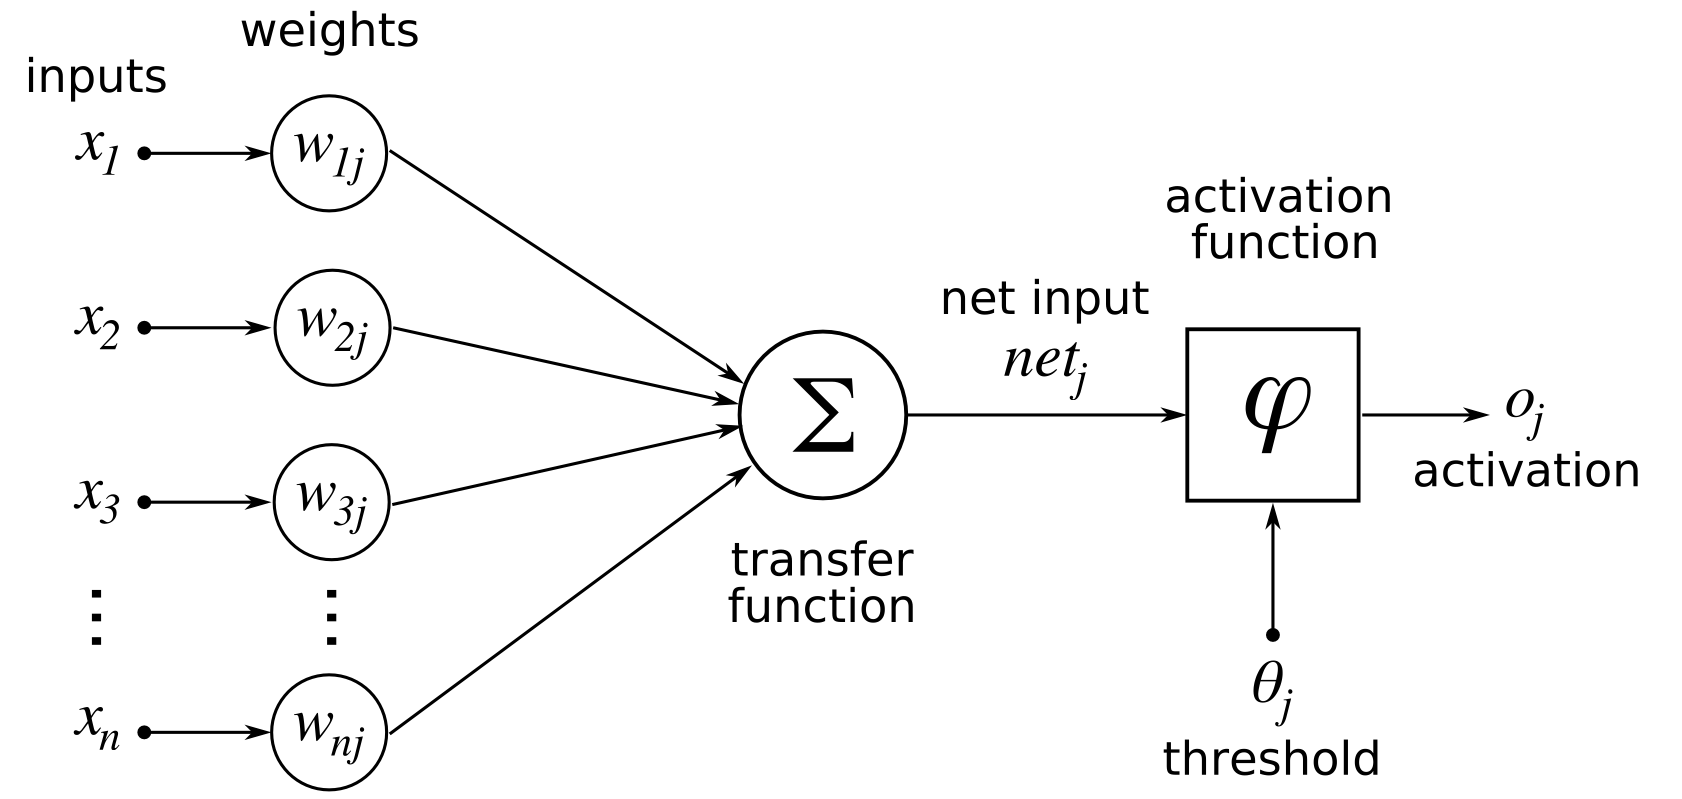
\includegraphics[width=.8\linewidth]{figures/ArtificialNeuronModel.png}
    \caption{Esempio di neurone artificiale \cite{wiki:xxx}}
    \label{fig:AN}
\end{figure}

A sua volta una rete neurale è composta da vari strati:
\begin{itemize}
    \item \textbf{Input Layer}: Questo è il primo strato della rete neurale
    e quello che riceve l'input esterno. Poiché la rete neurale
    è un modello matematico, l'input dovrà essere
    un vettore numerico. Questo vale anche se l'input da esaminare
    è una stringa di caratteri, come nel nostro caso.
    \item \textbf{Hidden Layer}: Questo è lo strato intermedio della rete neurale in cui avviene
    il processo di apprendimento.
    Questo strato elabora gli input ricevuti dallo strato precedente
    modificando i pesi. Si possono avere anche più hidden layers
    \item \textbf{Output Layer}: Questo è l'ultimo strato della rete neurale.
    Fornisce i risultati finali ottenuti dalla rete neurale. Questo strato
    può essere composto anche da un solo neurone che fornisce
    un output binario (0 o 1) come sarà nel nostro caso(DGA o non DGA)
\end{itemize}

\begin{figure}
    \centering
    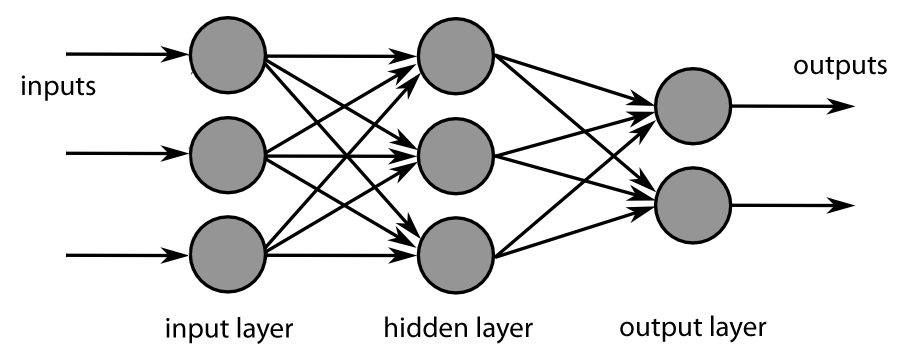
\includegraphics[width=.8\linewidth]{figures/MultiLayerNeuralNetwork.png}
    \caption{Esempio di rete neurale \cite{wiki:001}}
    \label{fig:ANN}
\end{figure}

Abbiamo inoltre vari tipi di reti neurali:
\begin{itemize}
    \item \textbf{Reti Neurali Feedforward}: Una rete Feedforward
    elabora le informazioni in un solo verso. Non ha né cicli
    né memoria delle informazioni passate. Questo tipo di rete
    è usato principalmente per riconoscimento di pattern o classificazioni
    \item \textbf{Reti Neurali Ricorrenti (RNN)}:
    A differenza di una rete Feedforward, in una RNN 
    i neuroni possono andare anche a formare dei cicli. 
    Questo permette alla rete di avere una specie di memoria
    e quindi di ricordare le informazioni passate. Usata
    per esempio per traduzione automatica o riconoscimento vocale.
    \item \textbf{Reti Neurali Convoluzionali (CNN)}:
\end{itemize}


\subsection{LSTM}

TODO

\chapter{Progetto}
\section{Obiettivi}
Il progetto ha come obiettivo quello di sviluppare un sistema
di rilevamento di domini generati da \acrshort{DGA} tramite
l'uso di tecniche di Machine Learning. 

Per il dataset di addestramento ho usato un dataset fornito dall'azienda 
Flashstart che contiene circa 5600 domini generati da \acrshort{DGA}.
A questo ho aggiunto un dataset di circa 5600 domini benigni
presi dal database di Cloudflare aggiornato
al 12 maggio 2025\cite{cloudflare_domains}


\section{Some cool topic}

\chapter{Contribution}

You may also put some code snippet (which is NOT float by default), eg: \cref{lst:random-code}.

\lstinputlisting[float,language=Java,label={lst:random-code}]{listings/HelloWorld.java}

\section{Fancy formulas here}

%----------------------------------------------------------------------------------------
% BIBLIOGRAPHY
%----------------------------------------------------------------------------------------

\backmatter

\bibliographystyle{IEEEtran} %prima era alpha
\bibliography{bibliography}

\begin{acknowledgements} % this is optional
Optional. Max 1 page.
\end{acknowledgements}

\end{document}
